%\documentclass{article}
%\usepackage{graphicx,subfigure}
%\begin{document}

\begin{figure}[h]
  \centering
   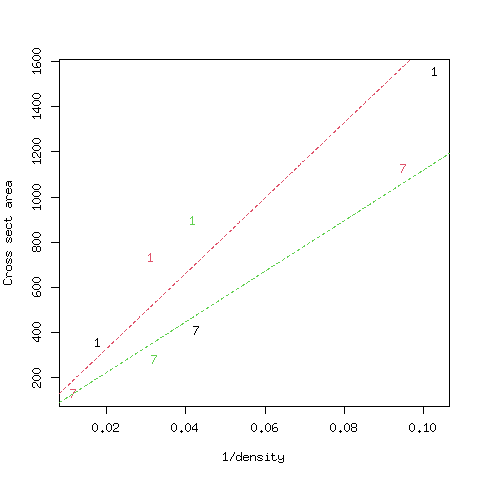
\includegraphics[width=0.9\textwidth]{DC1955/expt2reg.png}
  \caption{Plot of breed means for reciprocal of follicle density and fibre cross sectional area from Daly and Carter(1955)~\cite{daly:55} experiment 2.  The red lines are linear regressions  with zero intercept fitted to breed means for period 1 ({\em ad lib} nutrition. The green lines are linear regressions with zero intercept fitted to breed means for period 7 (restricted nutrition).}
  \label{fig:dcexpt2reg}
\end{figure}

%\end{document}

